\documentclass{beamer}


\usetheme{Warsaw}
\usecolortheme{crane}


\title{Boolean Algebra}
\subtitle{Mathematical Methods in the Physical Sciences}
\author{Steve Mazza}
\institute[Naval Postgraduate School]
{ 
    Naval Postgraduate School \\
    Monterey, CA \\
    
\includegraphics[height=3cm]{images/NPS_logo.jpg}
}
\date {SE3030, Winter/2014 \\ Quantitative Methods of Systems Engineering}
\subject{Quantitative Methods of Systems Engineering}


\begin{document}

\frame{\titlepage}


\frame{{Introduction}
    \begin{columns}[c]
    \column{.5\textwidth}
    In 1854 George Boole introduced a 2-state algebra designed to solve logic problems.  Today this algebra is at the heart of network and computer science.
    \column{.5\textwidth}
    \begin{center}
    	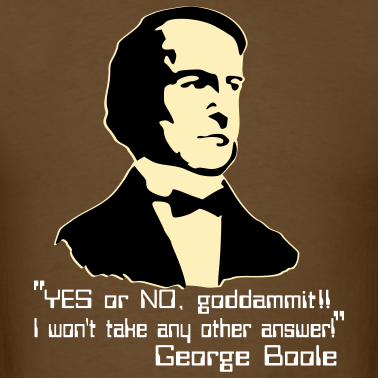
\includegraphics[scale=0.4]{images/boolean-algebra.png}
    \end{center}
    \end{columns}
}


\frame{{Basic Gates}
	\framesubtitle{NOT Gate}
	Receives input $x$ and produces $x'$ where
	\[
	x' = \left\{ 
	\begin{array}{rl}
		1 &\mbox{ if $x=0$} \\
  		0 &\mbox{ if $x=1$}
       	\end{array} \right.
	\]
	The output is the \emph{compliment} of the input.
    	\begin{columns}[c]
    	\column{.5\textwidth}
    	\begin{center}
    	\begin{tabular}{c c}
 		 $x$ & $x'$ \\
 		 \hline
 		 1 & 0 \\
 		 0 & 1 \\
	\end{tabular}
	\end{center}
    	\column{.5\textwidth}
    		\begin{center}
    			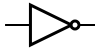
\includegraphics[scale=1]{images/100px-NOT_ANSI.png}
    		\end{center}
    	\end{columns}
}


\frame{{Basic Gates}
	\framesubtitle{AND Gate}
	Receives input $x_1$ and $x_2$ and produces $(x_1\wedge x_2)$ where
	\[
	(x_1\wedge x_2) = \left\{ 
	\begin{array}{rl}
		1 &\mbox{ if $x_1=x_2=1$} \\
  		0 &\mbox{ otherwise}
       	\end{array} \right.
	\]
	There may be more than two inputs but the there is always one output.
    	\begin{columns}[c]
    	\column{.5\textwidth}
    	\begin{center}
    	\begin{tabular}{c c c}
 		 $x_1$ & $x_2$ & $(x_1\wedge x_2)$ \\
 		 \hline
 		 0 & 0 & 0 \\
 		 0 & 1 & 0 \\
 		 1 & 0 & 0 \\
 		 1 & 1 & 1
	\end{tabular}
	\end{center}
    	\column{.5\textwidth}
    		\begin{center}
    			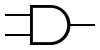
\includegraphics[scale=1]{images/100px-AND_ANSI.png}
    		\end{center}
    	\end{columns}
}


\frame{{Basic Gates}
	\framesubtitle{OR Gate}
	Receives input $x_1$ and $x_2$ and produces $(x_1\vee x_2)$ where
	\[
	(x_1\vee x_2) = \left\{ 
	\begin{array}{rl}
		1 &\mbox{ if $x_1=1$ or $x_2=1$} \\
  		0 &\mbox{ otherwise}
       	\end{array} \right.
	\]
	There may be more than two inputs but the there is always one output.
    	\begin{columns}[c]
    	\column{.5\textwidth}
    	\begin{center}
    	\begin{tabular}{c c c}
 		 $x_1$ & $x_2$ & $(x_1\wedge x_2)$ \\
 		 \hline
 		 0 & 0 & 0 \\
 		 0 & 1 & 1 \\
 		 1 & 0 & 1 \\
 		 1 & 1 & 1
	\end{tabular}
	\end{center}
    	\column{.5\textwidth}
    		\begin{center}
    			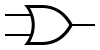
\includegraphics[scale=1]{images/100px-OR_ANSI.png}
    		\end{center}
    	\end{columns}
}


\frame{{Negated and Exclusive Gates}
	\framesubtitle{NOR Gate}
	Receives input $x_1$ and $x_2$ and produces $(x_1\vee x_2)'$ where
	\[
	(x_1\vee x_2)' = \left\{ 
	\begin{array}{rl}
		1 &\mbox{ if $x_1=x_2=0$} \\
  		0 &\mbox{ otherwise}
       	\end{array} \right.
	\]
	There may be more than two inputs but the there is always one output.
    	\begin{columns}[c]
    	\column{.5\textwidth}
    	\begin{center}
    	\begin{tabular}{c c c}
 		 $x_1$ & $x_2$ & $(x_1\wedge x_2)'$ \\
 		 \hline
 		 0 & 0 & 1 \\
 		 0 & 1 & 0 \\
 		 1 & 0 & 0 \\
 		 1 & 1 & 0
	\end{tabular}
	\end{center}
    	\column{.5\textwidth}
    		\begin{center}
    			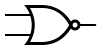
\includegraphics[scale=1]{images/100px-NOR_ANSI.png}
    		\end{center}
    	\end{columns}
}


\frame{{Negated and Exclusive Gates}
	\framesubtitle{NAND Gate}
	Receives input $x_1$ and $x_2$ and produces $(x_1\wedge x_2)'$ where
	\[
	(x_1\wedge x_2)' = \left\{ 
	\begin{array}{rl}
		1 &\mbox{ if $x_1=0$ or $x_2=0$} \\
  		0 &\mbox{ otherwise}
       	\end{array} \right.
	\]
	There may be more than two inputs but the there is always one output.
    	\begin{columns}[c]
    	\column{.5\textwidth}
    	\begin{center}
    	\begin{tabular}{c c c}
 		 $x_1$ & $x_2$ & $(x_1\wedge x_2)'$ \\
 		 \hline
 		 0 & 0 & 1 \\
 		 0 & 1 & 1 \\
 		 1 & 0 & 1 \\
 		 1 & 1 & 0
	\end{tabular}
	\end{center}
    	\column{.5\textwidth}
    		\begin{center}
    			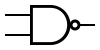
\includegraphics[scale=1]{images/100px-NAND_ANSI.png}
    		\end{center}
    	\end{columns}
}


\frame{{Negated and Exclusive Gates}
	\framesubtitle{XOR Gate}
	Receives input $x_1$ and $x_2$ and produces $(x_1\oplus x_2)$ where
	\[
	(x_1\oplus x_2) = \left\{ 
	\begin{array}{rl}
		1 &\mbox{ if only $x_1=0$ or only $x_2=1$} \\
  		0 &\mbox{ otherwise}
       	\end{array} \right.
	\]
	There may be more than two inputs but the there is always one output.
	The XNOR gate implements the logical expressions: $x_1 \cdot \overline{x_2} + \overline{x_1} \cdot x_2$ and $(x_1 + x_2) \cdot \overline{x_1 \cdot x_2}$.
    	\begin{columns}[c]
    	\column{.5\textwidth}
    	\begin{center}
    	\begin{tabular}{c c c}
 		 $x_1$ & $x_2$ & $(x_1\oplus x_2)$ \\
 		 \hline
 		 0 & 0 & 0 \\
 		 0 & 1 & 1 \\
 		 1 & 0 & 1 \\
 		 1 & 1 & 0
	\end{tabular}
	\end{center}
    	\column{.5\textwidth}
    		\begin{center}
    			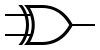
\includegraphics[scale=1]{images/100px-XOR_ANSI.png}
    		\end{center}
    	\end{columns}
}


\frame{{Negated and Exclusive Gates}
	\framesubtitle{XNOR Gate}
	Receives input $x_1$ and $x_2$ and produces $(x_1\oplus x_2)'$ where
	\[
	(x_1\oplus x_2)' = \left\{ 
	\begin{array}{rl}
		1 &\mbox{ if $x_1=x_2$} \\
  		0 &\mbox{ otherwise}
       	\end{array} \right.
	\]
	There may be more than two inputs but the there is always one output. 
	The XNOR gate implements the logical expression: $x_1 \cdot x_2 + \overline{x_1} \cdot \overline{x_2}$.
    	\begin{columns}[c]
    	\column{.5\textwidth}
    	\begin{center}
    	\begin{tabular}{c c c}
 		 $x_1$ & $x_2$ & $(x_1\oplus x_2)'$ \\
 		 \hline
 		 0 & 0 & 1 \\
 		 0 & 1 & 0 \\
 		 1 & 0 & 0 \\
 		 1 & 1 & 1
	\end{tabular}
	\end{center}
    	\column{.5\textwidth}
    		\begin{center}
    			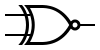
\includegraphics[scale=1]{images/100px-XNOR_ANSI.png}
    		\end{center}
    	\end{columns}
}


\frame{{Combinatorial Circuit}
	%TODO
}


\frame{{Boolean Expression}
	%TODO
}


\frame{{Equivalent Combinatorial Circuits}
	%TODO
}


\frame{{Boolean Algebra}
	%TODO
}


\frame{{Dual of a Statement}
	%TODO
}


\frame{{Boolean Function}
	%TODO
}


\frame{{Various Normal Forms}
	%TODO
}


\frame{{Questions?}
	\begin{center}
		
\includegraphics[width=.7\textwidth]{images/fin.png}
	\end{center}
}

\end{document}
